
Il mio lavoro inizia con lo studio e l'utilizzo del formato
\textbf{SBML} (\textbf{S}ystems \textbf{B}iology \textbf{M}arkup 
\textbf{L}anguage). 

Questo formato permette di rappresentare informazioni seguendo uno
schema gerarchico, basato su XML. Questo formato \`e orientato alla
descrizione di sistemi in cui entit\`a biologiche sono oggetto di
manipolazioni eseguite da processi nel corso del tempo, pertanto
facilita la codifica di modelli computazionali di processi biologici,
ad esempio \emph{metabolic networks, cell-signaling pathways,
  regulatory networks} e molti altri. In particolare, le
\emph{metabolic network} sono oggetto del mio elaborato.
\\\\
Nella prossima sezione descrivo brevemente il contesto scientifico che
ospita il nostro problema, introducendo i concetti reali oggetto delle
astrazioni che ho costruito e implementato nel mio codice.

\section{Metabolic networks, enzimes and pathways}

Prima di definire cosa \`e una \emph{metabolic network} dobbiamo
introdurre i seguenti concetti.

Una \emph{metabolic pathway} \`e una sequenza di reazioni chimiche che
si verificano all'interno di una cellula. Dal punto di vista
matematico, possiamo vedere una metabolic pathway come una sequenza di
funzioni $reaction_{i}$ tali che:
\begin{displaymath}
reaction_{i} : 2^{Molecules} \rightarrow 2^{Molecules}
\end{displaymath}
Ognunga di queste funzioni, avendo in input un insieme di molecole,
esegue delle trasformazioni su queste e produce come output, il
risultato delle trasformazioni svolte sottoforma di insieme di
molecole. Questo output pu\`o essere utilizzato come input per
$reaction_{i+1}$, concatenando quanto si voglia le trasformazioni.
\\\\
Ogni reazione chimica \`e regolata da alcuni \emph{enzymes}.

Un \emph{enzyme} \`e una proteina che gestisce la frequenza e la
velocit\`a di una reazione chimica. Le molecole a cui si applica la
reazione vengono identificate con il termine \emph{substrates} (o
\emph{reactants} usando la terminologia SBML), mentre i prodotti della
reazione vengono indentificati con il termine \emph{products} (anche la
terminologia SBML usa questo identificatore).

Durante l'esecuzione di una reazione chimica, ogni \emph{enzyme}
agisce da \emph{catalyst}, ovvero non viene consumato nella reazione
e, quindi, pu\`o partecipare in pi\`u di una reazione.

L'insieme di \emph{enzymes} "guida" e determina l'insieme di
\emph{pathways} che possono occorrere nella cellula, in quanto una
reazione chimica su un substrato pu\`o avvenire se e solo se lo strato
attivo del substrato complementa quello dell'enzima.

Adesso possiamo definire una \emph{metabolic network} come collezione
di \emph{metabolic pathways}.
\\\\
Nella prossima sezione vedremo quali di questi concetti sono necessari
al mio lavoro, cercando di metterli in relazione con le astrazioni
definite dal formato SBML.

\section{Model necessary real objects in SBML}

Adesso che abbiamo alcuni concetti reali possiamo iniziare a mapparli
sulle nostre astrazioni, la prima delle quali \`e il mezzo di
comunicazione SBML.

Nella precedente sezione abbiamo introdotto alcuni concetti che non
sono influenti sul nostro studio, per cui trattiamo solo quelli
inerenti al lavoro che ho sviluppato (molti dei concetti che noi non
usiamo sono comunque modellabili in SBML).
\\\\
Le unit\`a atomiche definibili con SBML sono le \emph{specie}. Una
specie rappresenta il concetto di molecola (appartenente ad almeno un
\emph{substrate}). Possiamo modellare molti attributi con un oggetto
di tipo specie ma, ai nostri fini, due sono quelli che usiamo:
\begin{itemize}
\item \emph{identifier}, che permette di assegnare una etichetta univoca
alla specie all'interno di tutto il modello SBML
\item \emph{compartment}, che permette di assegnare ad una specie il
compartimento della cellula dove risiede (in tutti gli esempi che
abbiamo avuto modo di testare il compartimento \`e sempre il
citoplasma).
\end{itemize}

Un altro concetto fondamentale \`e quello di \emph{chemical reaction},
codificato in SBML con:
\begin{itemize}
\item \emph{reactants}, insieme di \emph{species}, che modellano il
  \emph{substrate} della reazione.
\item \emph{products}, insieme di \emph{species}, che modellano i
  prodotti della reazione.
\end{itemize}
Inoltre \`e necessario modellare il concetto di reazione
reversibile, il quale viene catturato in SBML dal flag
\emph{reversible}.
\\\\
Questo \`e quello che ci serve per iniziare ad analizzare il modello
SBML: ricercheremo l'insieme di reazioni descritte e, per ogni
reazione, analizzeremo l'insieme dei \emph{reactants} e dei
\emph{products} per costruire un nostro modello sul quale implementare
i nostri algoritmi.
\\\\
Nella prossima sezione descriveremo le regole che abbiamo utilizzato
per costruire, dato in input un modello SBML, il nostro modello
dati.

\section{SBML model $\rightarrow$ Our model}

Abbiamo la necessit\`a di modellare i concetti espressi in formato
SBML con un nostro modello in quanto ci permette di ridurre la
complessit\`a delle informazioni e ci permette di applicare in modo
semplice molti algoritmi presi dalla teoria dei grafi.

Senza questo nostro modello la trattazione del problema sarabbe molto
complicata e non ci permetterebbe di arrivare a dei
risultati\footnote{Qui potrebbe essere il caso di inserire
  l'osservazione che fece Andrea sugli ipergrafi, che renderebbero il
  problema NP-completo. Mi ricordo bene?}.
\\\\
Il nostro modello \`e essenzialmente un grafo orientato, la cui
caratteristica \`e quella di catturare l'idea dei nodi \emph{black} e
nodi \emph{white}, definiti nell'articolo Crescenzi-Marino
\footnote{aggiungere qua riferimento bibliografico all'articolo
  "Telling Stories"}, componenti essenziali per l'astrazione di \emph{story}.

Per costruire questo modello usiamo questo insieme di regole:
\begin{itemize}
\item due specie sono uguali se hanno uguale identificatore ed uguale
  compartimento. Questa regola \`e necessaria per evitare una
  esplosione di nodi del nostro modello, in quanto se $a \in
  reactants(r) \wedge a' \in reactants(r'), a = a' \wedge r \not = r'$
  si creassero due nodi distinti per $a, a'$, non si avrebbero
  informazioni significative in quanto il grafo degenerebbe ad un
  insieme di sottografi, ognuno rappresentante una reazione. Quindi
  una specie non \`e identificata dalle reazioni in cui appare.
\item data una reazione non-reversibile $r$ tale che:
  \begin{displaymath}
    \begin{split} 
      reactants(r) &= \{ r_{1}, \ldots, r_{n} \} \\
      products(r) &= \{ p_{1}, \ldots, p_{m} \}
    \end{split}
  \end{displaymath}
  allora il nostro modello sar\`a uguale al grafo che codifica la
  relazione $reactants(r) \times products(r)$. Ad esempio, con
  $reactants(r) = \{ a, b, c, d \}$ e $products(r) = \{a, e, f\}$
  otteniamo:

\begin{figure}[!htb]
\centering
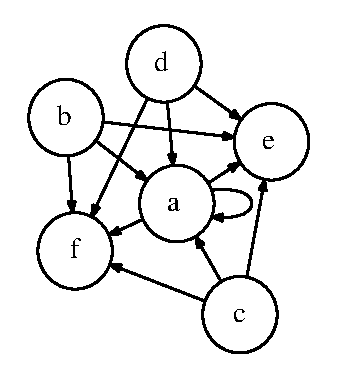
\includegraphics{images/non-reversible-reaction-example.dot.eps}
\end{figure}
supponendo che la specie $a$ appartenente ad entrambi gli
insiemi sia la stessa (ovvero se $\exists a': a = a' \rightarrow id(a) =
id(a') \wedge compart(a) = compart(a')$).

\item data una reazione reversibile $r$ tale che:
  \begin{displaymath}
    \begin{split} 
      reactants(r) &= \{ r_{1}, \ldots, r_{n} \} \\
      products(r) &= \{ p_{1}, \ldots, p_{m} \}
    \end{split}
  \end{displaymath}
  allora il nostro modello sar\`a uguale al grafo che codifica la
  relazione $(reactants(r) \times products(r)) \cup (products(r)
  \times reactants(r))$. Ad esempio, con $reactants(r) = \{ a, b, c, d
  \}$ e $products(r) = \{a, e, f\}$ otteniamo:

\begin{center}
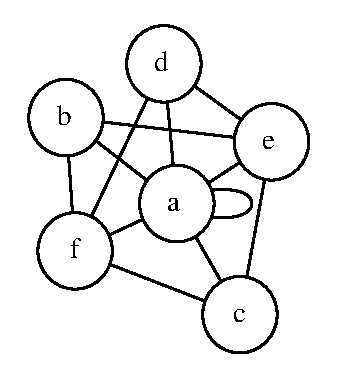
\includegraphics{images/reversible-reaction-example.dot.eps}
\end{center}
supponendo che la specie $a$ appartenente ad entrambi gli
insiemi sia la stessa (ovvero se $\exists a': a = a' \rightarrow id(a) =
id(a') \wedge compart(a) = compart(a')$).

\end{itemize}
